Podemos establecer una relación entre las coordenadas rectangulares y las polares mediante la construcción de un punto en un plano bidimensional, como se muestra en la siguiente ilustración:

\begin{figure}[H]
  \centering
  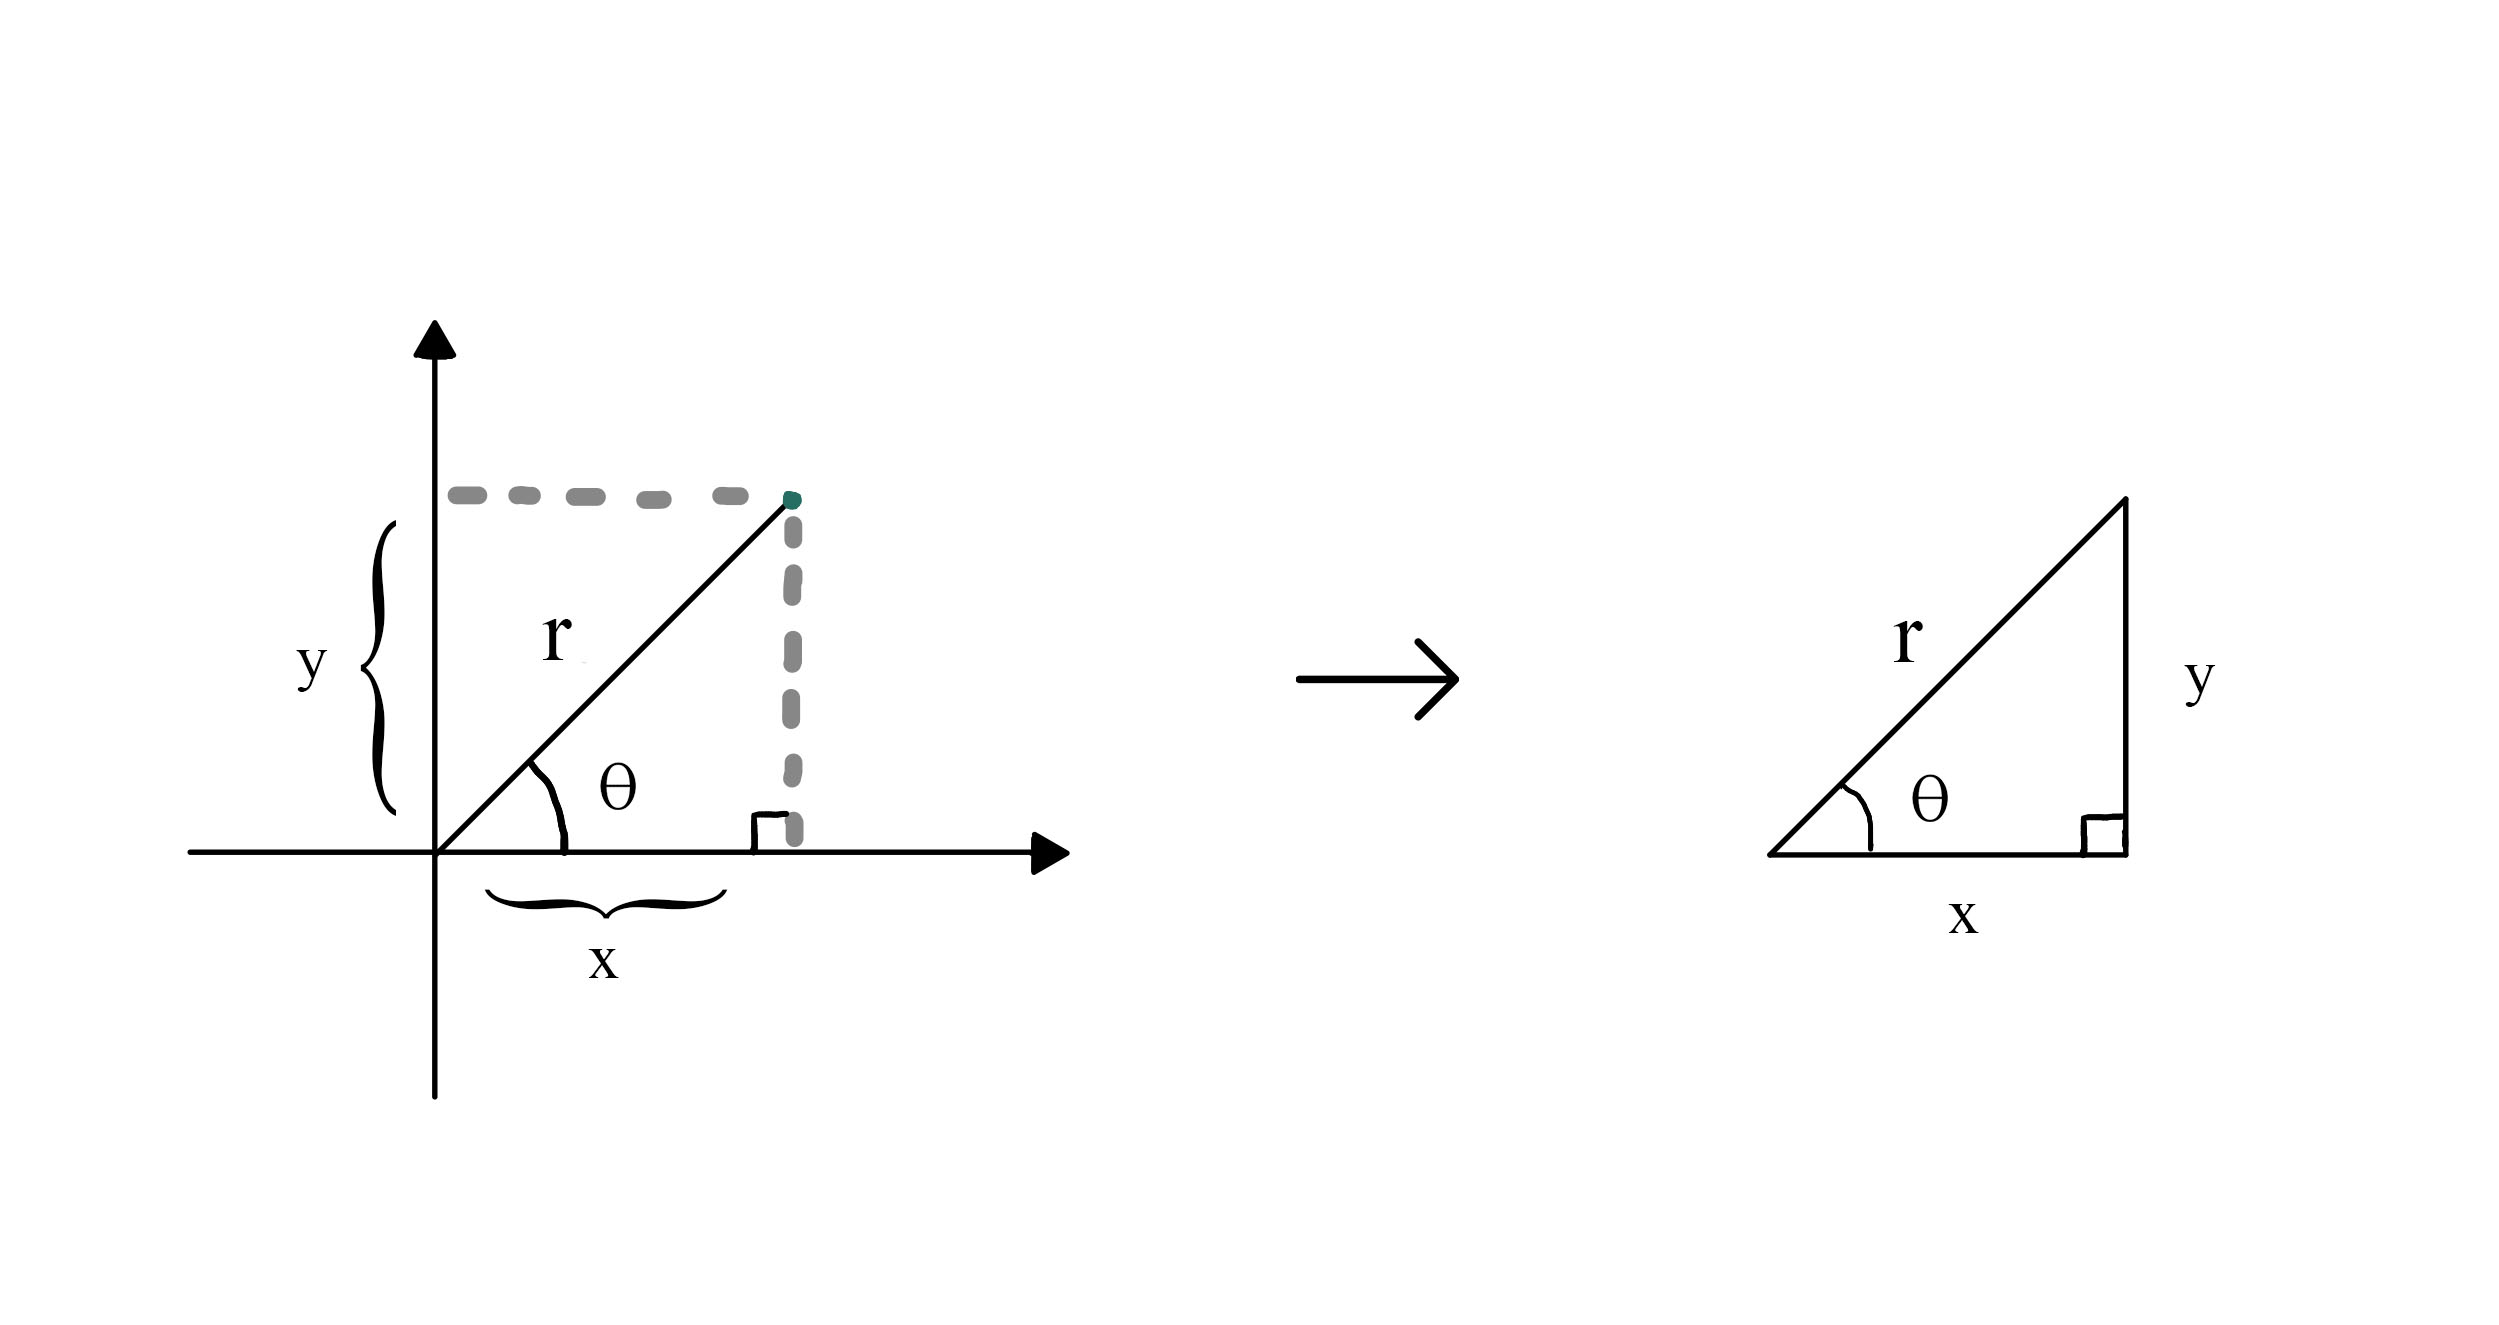
\includegraphics[width=11.17cm, height=5.67cm]{img/graph/relacion_r}
  \caption{Relación de coordenadas rectangulares y polares.}
  \label{relacion_de_coordenadas}
\end{figure}

Donde $r$ representa la distancia desde el origen hasta el punto, formándose un triángulo rectángulo con ángulo $\theta$.
